\section{Связь между доверительными интервалами и проверками гипотез}
Утверждение о том, что $(\widehat{\theta}_{\text{lo}},\  \widehat{\theta}_{\text{up}})$ это $1 - 2 \alpha$ доверительный интервал для $\theta$ можно интерпретировать и по другому. Предположим, что настоящее значение $\theta$ было равно $\widehat{\theta}_{\text{lo}}$
\begin{gather}\label{12.12}
\widehat{\theta}^{*} \sim \mathrm{N}(\hat{\theta}_{\text{lo}}, \ \text{se}^{2}).
\end{gather}

Мы использовали обозначение $\widehat{\theta}^{*}$ для обозначения случайной величины, чтобы избежать путаницы с наблюдаемой оценкой $\widehat{\theta}$. Величину $\widehat{\theta}_{\text{lo}}$ в (\ref{12.12}) считаем фиксированной, случайным является только $\widehat{\theta}^{*}$. Легко заметить, что вероятность того, что $\widehat{\theta}^{*}$ превышает фактическую оценку $\widehat{\theta}$, равна $\alpha$
\begin{gather}\label{12.13}
\text{Prob}_{\widehat{\theta}_{\text{lo}}} \left\{ \widehat{\theta}^{*} \ge \widehat{\theta}  \right\} = \alpha.
\end{gather}
Тогда для любого значения $\theta$ меньшего чем $\widehat{\theta}_{\text{lo}}$ получаем
$\widehat{\theta}$, равна $\alpha$
\begin{gather}\label{12.14}
\text{Prob}_{\theta} \left\{\widehat{\theta}^{*} \ge \widehat{\theta}  \right\} < \alpha \ \ \ \ [\text{для} \  \theta < \widehat{\theta}_{\text{lo}}].
\end{gather}
При вычислении вероятности в (\ref{12.14}) $\widehat{\theta}$ зафиксировано, а значение $\widehat{\theta}^{*}$ случайное, $\widehat{\theta}^{*} \sim \mathrm{N}(\widehat{\theta}_{\text{lo}}, \ \text{se}^{2})$, см. (\ref{12.2}). Так же для любого значения $\theta$ большего верхнего предела $\widehat{\theta}_{\text{up}}$
\begin{gather}\label{12.15}
\text{Prob}_{\widehat{\theta}_{\text{lo}}}\left\{\widehat{\theta}^{*} \le \widehat{\theta}  \right\} < \alpha \ \ \ \ [\text{для} \  \theta > \widehat{\theta}_{\text{up}}].
\end{gather}
Идею доверительного интервала $(\widehat{\theta}_{\text{lo}}, \ \widehat{\theta}_{\text{up}})$ можно сформулировать в терминах (\ref{12.14}) --- (\ref{12.15}). Мы выбираем маленькую вероятность $\alpha$ которая является «уровнем занчимости». И считаем, что значения параметра $\theta$ которые меньше $\widehat{\theta}_{\text{lo}}$ являются неправдоподобными, потому что их вероятность меньше $\alpha$ чем наблюдения такой же большой оценки, как  наблюдаемая (\ref{12.14}). Cчитаем что значения $\theta$ больше $ \widehat{\theta}_{\text{up}}$ недопустимы, потому что они дают вероятность меньше $\alpha$ чем наблюдения такой же малой оценки, как наблюдаемая, (\ref{12.15}).(????) Подведём итог: \textit{$1 - 2 \alpha$ доверительный интервал $(\widehat{\theta}_{\text{lo}}, \ \widehat{\theta}_{\text{up}})$ --- это набор вероятных значения $\theta$ наблюдаемых $\widehat{\theta}$, эти значения не исключаются ни одним из тестов правдоподобия (\ref{12.14}) или (\ref{12.15}).}
\begin{figure}[H]
\center{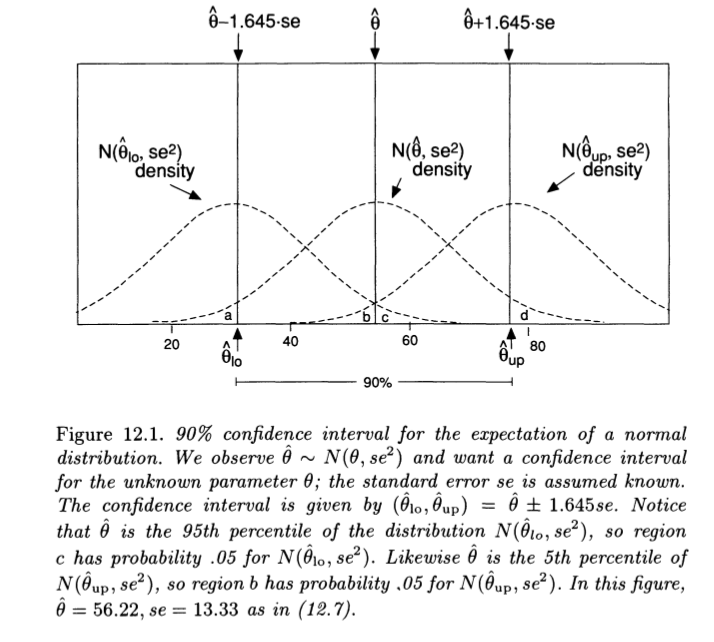
\includegraphics[width=1 \linewidth]{12.1.png}}
\end{figure}
Cитуация проиллюстрирована на рисунке 12.1. Мы предполагаем, что $\widehat{\theta} \sim \mathrm{N}(\theta, \ \text{se}^{2})$, как в (\ref{12.8}), положим 
$ \alpha = 0.05, 1-2\alpha = 0.90.$ Наблюдая $\widehat{\theta}$, $90\%$ доверительный интервал (\ref{12.10}) имеет границы
\begin{gather}\label{12.16}
\widehat{\theta}_{\text{lo}} = \widehat{\theta} - 1.645 \cdot\text{se}, \ \ \ \widehat{\theta}_{\text{up}} = \widehat{\theta} + 1.645 \cdot \text{se}
\end{gather}
Пунктирная кривая, достигающая максимальное значение в точке $\widehat{\theta}_{\text{lo}}$, является кривой плотности вероятности нормального распределения $ \mathrm{N}(\widehat{\theta}_{\text{lo}}, \  \text{se}^{2})$. 95-ый процентиль распределения $ \mathrm{N}(\widehat{\theta}_{\text{lo}}, \ \text{se}^{2})$ находится в точке $\widehat{\theta}$. Другими словами, область под кривой плотности распределения $ \mathrm{N}(\widehat{\theta}_{\text{lo}}, \ \text{se}^{2})$  справа от $\widehat{\theta}$, обозначенная буквой <<с>>, имеет площадь равную 0.05. Пунктирная кривая, максимум которой достигается в точке $\widehat{\theta}_{\text{up}}$, является кривой плотности вероятности $\mathrm{N}(\widehat{\theta}_{\text{up}}, \ \text{se}^{2})$;  $\widehat{\theta}$ это 5-ый процентиль распределения; а площадь области <<b>> равна 0.05. Проверки правдоподобия (\ref{12.14}) и (\ref{12.15}) также являются уровнями значимости для соответствующей \textit{проверки гипотезы}. Значение в (\ref{12.14}) - это уровень значимости для односторонней альтернативной гипотезы о том, что истинный параметр больше, чем  $\theta$, а (\ref{12.15)} - это уровень значимости для односторонней альтернативной гипотезы о том, что истинный параметр меньше $\theta$. Во многих ситуациях проверка гипотезы может быть проведена путем построения доверительного интервала и последующей проверки того, находится ли нулевое значение интервале. Проверка гипотез обсуждается в главах 15 и 16. 